%% ma: L11-B14-0017
%% lop: 11
%% chuong: 4
%% bai: 14
%% dang: 11.14.3
%% loai: TN4
%% muc: TH
%% dap_an: "B"
%% nguon: "tai-lieu-hoc-tap-mon-toan-lop-11-theo-chuong-trinh-giao-duc-pho-thong-2018.pdf (Lớp Toán Thầy Duy, Phạm Lê Duy, THPT Chu Văn An), Chương 4 Bài 5, Phần 1, Câu 12 (tr.529)"
%% kien_thuc: "Lớp 11 Bài 14 (phép chiếu song song)"
%% trang_thai: chinh-thuc
%% ghi_chu: "Bốn hình TikZ dựng lại theo hình gốc. Đã duyệt 03/11/2026."
\begin{ex}
Trong không gian, hình nào \textbf{không} phải là hình biểu diễn của hình chóp tam giác?
\begin{center}
\begin{minipage}{0.2\linewidth}\centering
\begin{tikzpicture}[scale=0.8]
\draw (0.71,2.73)--(0.00,0.87);
\draw (0.71,2.73)--(1.95,0.87);
\draw (0.71,2.73)--(1.45,0.04);
\draw (0.00,0.87)--(1.45,0.04);
\draw (1.45,0.04)--(1.95,0.87);
\draw[khuat] (0.00,0.87)--(1.95,0.87);
\end{tikzpicture}

\textbf{A.}
\end{minipage}\hfill
\begin{minipage}{0.2\linewidth}\centering
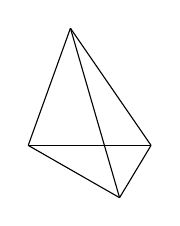
\begin{tikzpicture}[scale=0.8]
\draw (0.67,2.73)--(0.00,0.87);
\draw (0.67,2.73)--(1.95,0.87);
\draw (0.67,2.73)--(1.45,0.04);
\draw (0.00,0.87)--(1.45,0.04);
\draw (1.45,0.04)--(1.95,0.87);
\draw (0.00,0.87)--(1.95,0.87);
\end{tikzpicture}

\textbf{B.}
\end{minipage}\hfill
\begin{minipage}{0.2\linewidth}\centering
\begin{tikzpicture}[scale=0.8]
\draw (0.95,2.73)--(0.00,0.04);
\draw (0.95,2.73)--(2.85,0.04);
\draw (0.00,0.04)--(2.85,0.04);
\draw[khuat] (0.95,2.73)--(1.49,0.51);
\draw[khuat] (1.49,0.51)--(0.00,0.04);
\draw[khuat] (1.49,0.51)--(2.85,0.04);
\end{tikzpicture}

\textbf{C.}
\end{minipage}\hfill
\begin{minipage}{0.2\linewidth}\centering
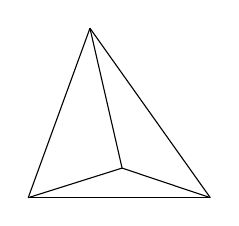
\begin{tikzpicture}[scale=0.8]
\draw (0.98,2.73)--(0.00,0.04);
\draw (0.98,2.73)--(2.89,0.04);
\draw (0.00,0.04)--(2.89,0.04);
\draw (0.98,2.73)--(1.49,0.51);
\draw (1.49,0.51)--(0.00,0.04);
\draw (1.49,0.51)--(2.89,0.04);
\end{tikzpicture}

\textbf{D.}
\end{minipage}\hfill
\end{center}
\choice{Hình A.}{\True Hình B.}{Hình C.}{Hình D.}
\loigiai{\sloppy Hình B vẽ tất cả các cạnh bằng nét liền, trong đó hai cạnh chéo nhau (cạnh đáy phía sau và cạnh bên phía trước) cắt nhau trên hình vẽ mà không có nét đứt cho cạnh bị che, nên không phải hình biểu diễn đúng của tứ diện. Hình A có cạnh khuất vẽ nét đứt; hình C có đỉnh khuất phía sau vẽ nét đứt; hình D có đỉnh đáy nằm phía trước nên mọi cạnh đều thấy: cả ba đều hợp lệ.}
\end{ex}
